% Native editable composition of three verified, unchanged IDE captures.
\begin{figure}[htbp]
\centering
\sbox0{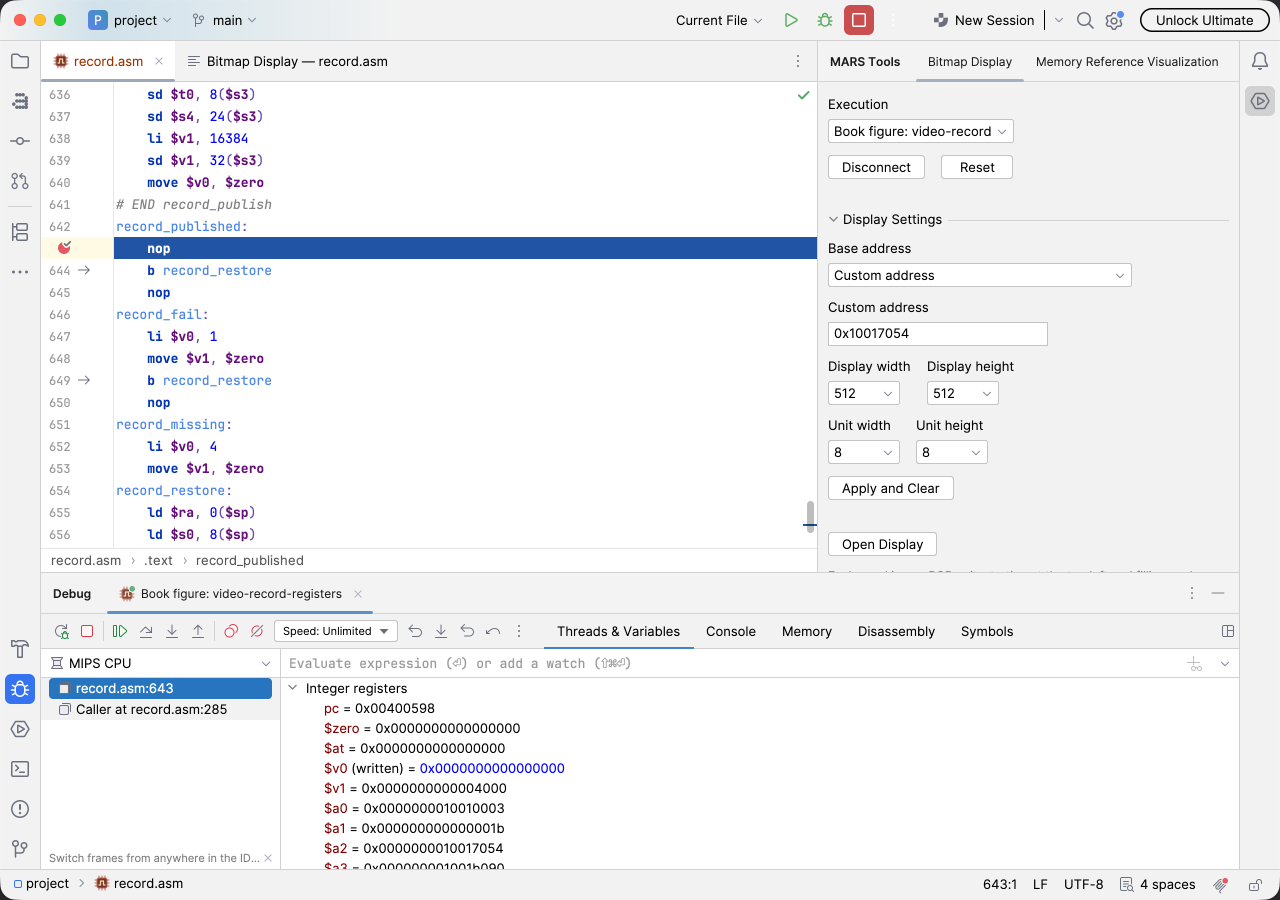
\includegraphics[artifact]{packages/034-lossless-video/captures/video-record-publication/registers.png}}
\sbox2{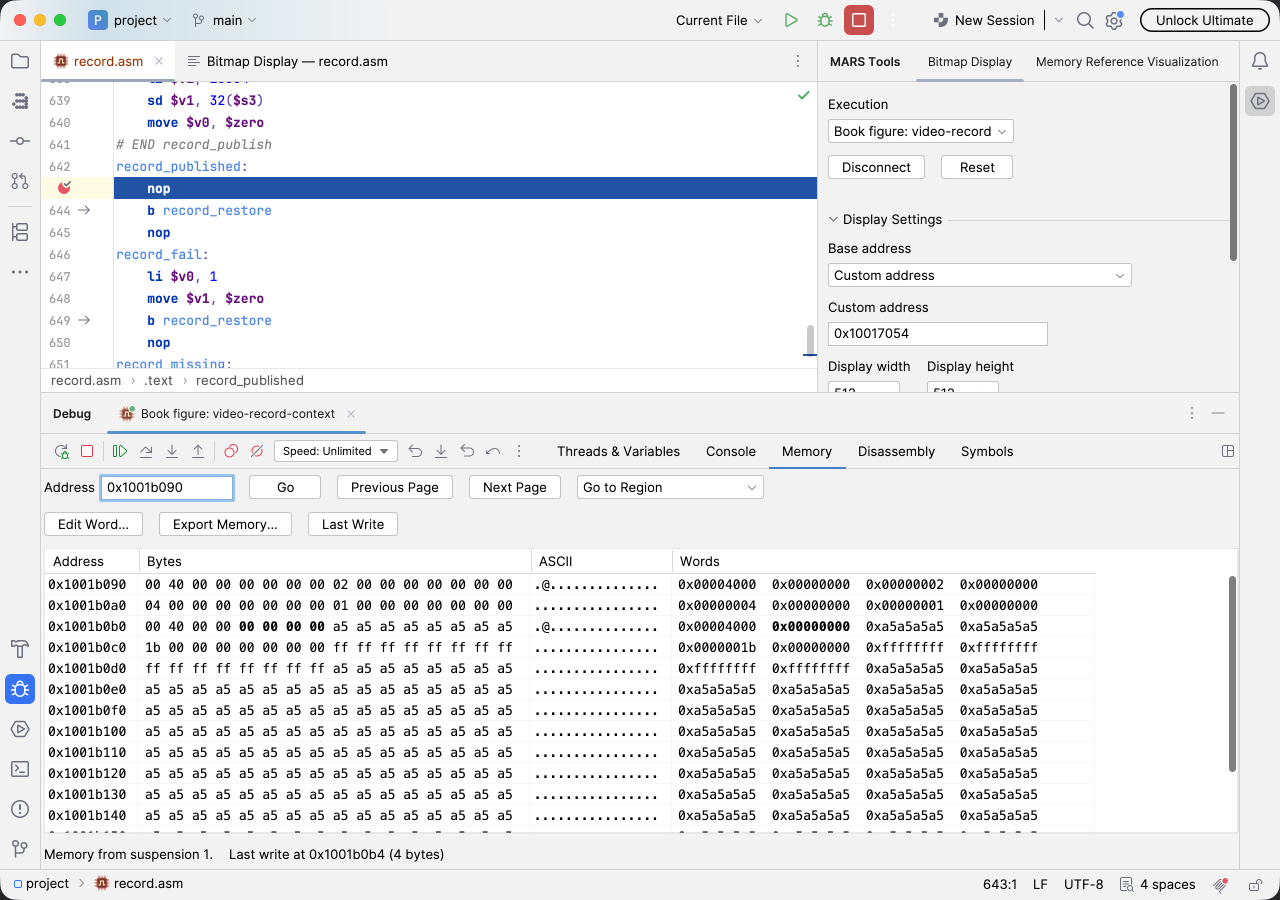
\includegraphics[artifact]{packages/034-lossless-video/captures/video-record-publication/context.png}}
\sbox4{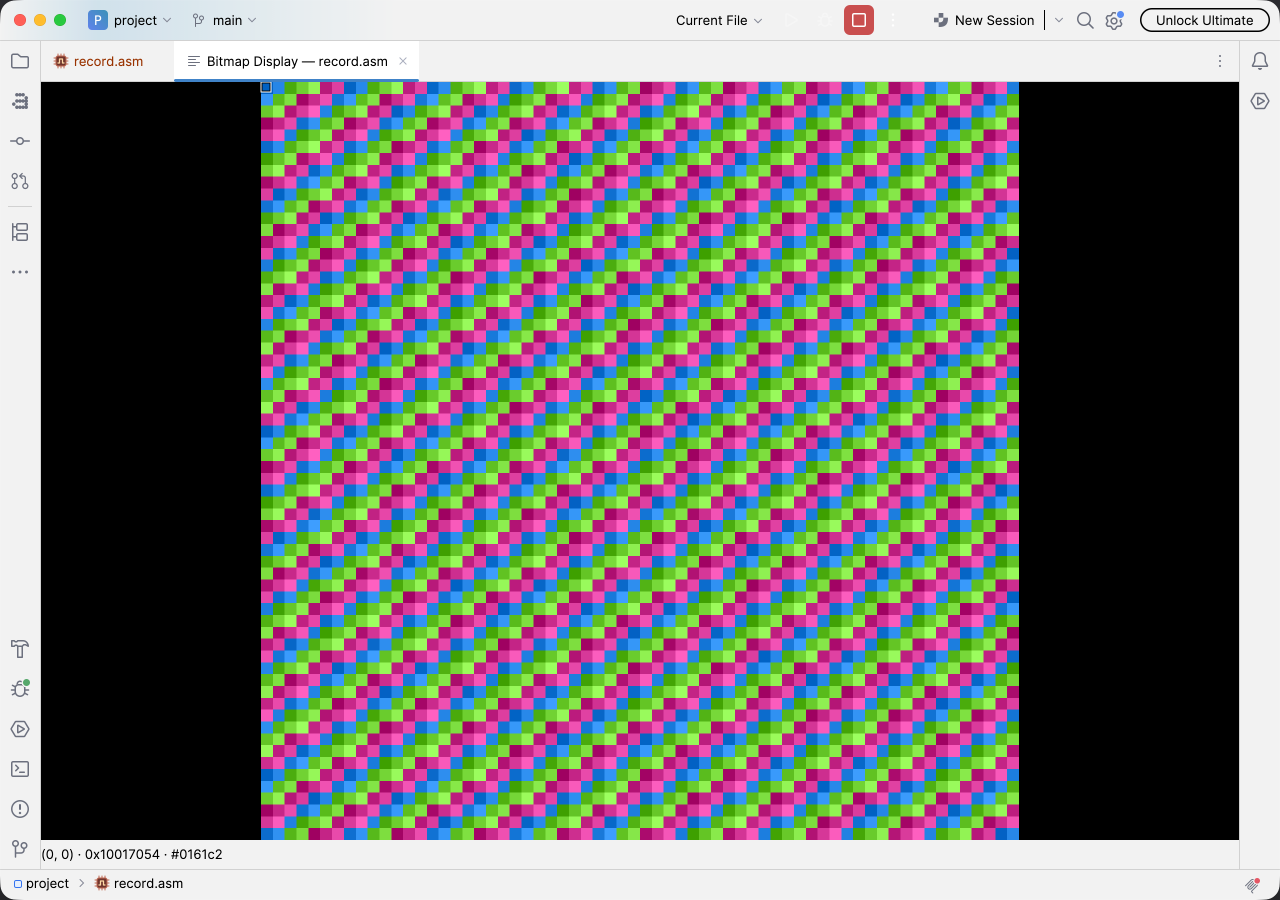
\includegraphics[artifact]{packages/034-lossless-video/captures/video-record-publication/bitmap.png}}
\edef\MARSrecordsourceLeft{\the\dimexpr0.036718750\wd0\relax}
\edef\MARSrecordsourceBottom{\the\dimexpr0.707777778\ht0\relax}
\edef\MARSrecordsourceRight{\the\dimexpr0.611718750\wd0\relax}
\edef\MARSrecordsourceTop{\the\dimexpr0.238888889\ht0\relax}
\edef\MARSrecordbitmapLeft{\the\dimexpr0.199218750\wd4\relax}
\edef\MARSrecordbitmapBottom{\the\dimexpr0.060000000\ht4\relax}
\edef\MARSrecordbitmapRight{\the\dimexpr0.199218750\wd4\relax}
\edef\MARSrecordbitmapTop{\the\dimexpr0.084444444\ht4\relax}
\edef\MARSrecordcontextLeft{\the\dimexpr0.520312500\wd2\relax}
\edef\MARSrecordcontextBottom{\the\dimexpr0.288888889\ht2\relax}
\edef\MARSrecordcontextRight{\the\dimexpr0.139843750\wd2\relax}
\edef\MARSrecordcontextTop{\the\dimexpr0.634444444\ht2\relax}
\edef\MARSrecordreturnsLeft{\the\dimexpr0.246093750\wd0\relax}
\edef\MARSrecordreturnsBottom{\the\dimexpr0.111111111\ht0\relax}
\edef\MARSrecordreturnsRight{\the\dimexpr0.553906250\wd0\relax}
\edef\MARSrecordreturnsTop{\the\dimexpr0.840000000\ht0\relax}
\begin{tikzpicture}[alt={Four annotated native IDE details at record_published, before its nop. Detail 1 marks the next instruction. Detail 2 shows the accepted 64 by 64 frame as repeating diagonal color bands. Detail 3 shows the context as little-endian low/high 32-bit word pairs: retained capacity 16384, next sequence 2, retained period 4, accepted kind 1, active bytes 16384, and the retained A5 suffix. Detail 4 shows success v0 equal to zero and v1 equal to 16384 bytes.}]
\node[anchor=north west,inner sep=0,font=\small\bfseries] (source-title) at (6mm,0) {Paused publication checkpoint};
\node[anchor=north west,inner sep=0] (source) at ([yshift=-1mm]source-title.south west) {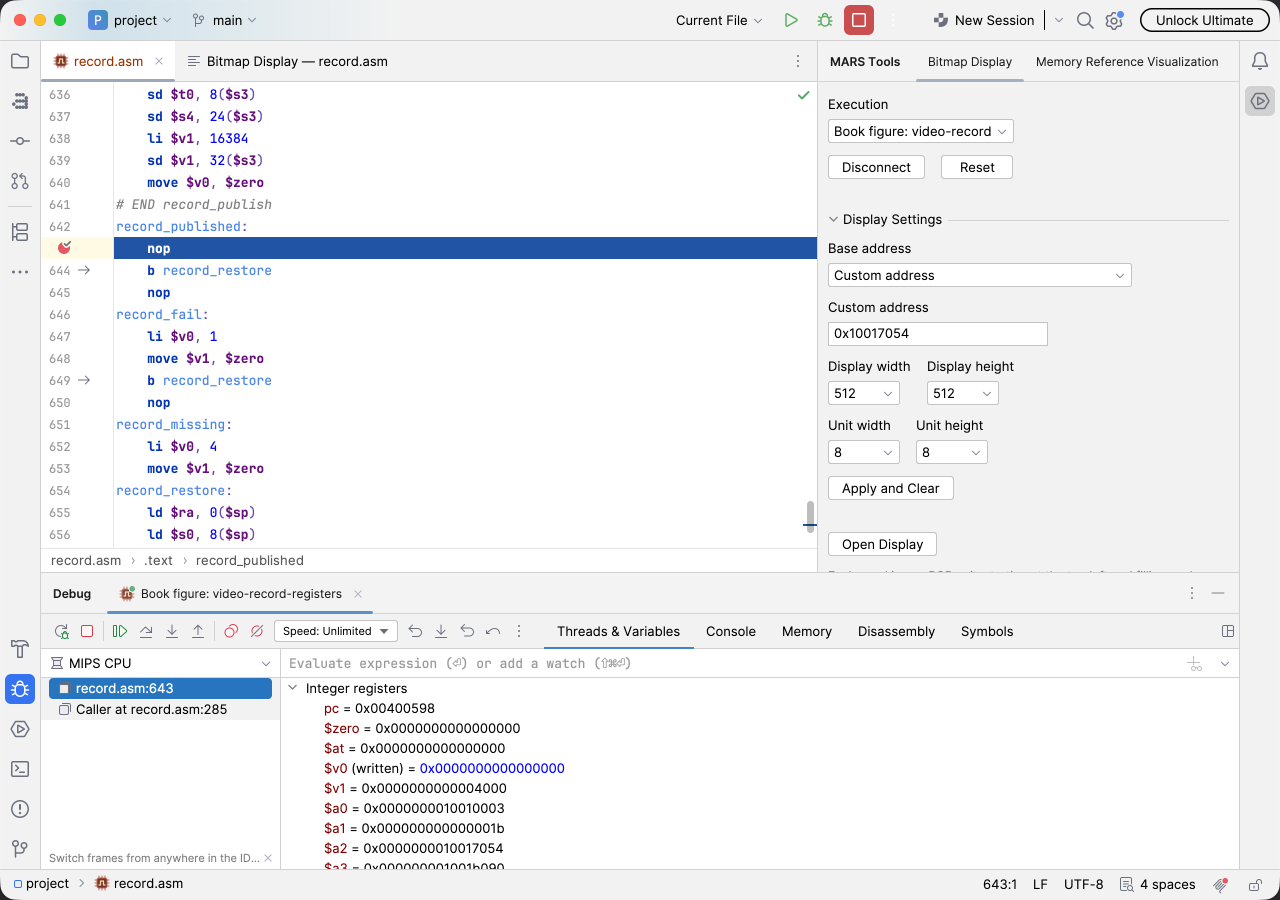
\includegraphics[width=0.7\linewidth,artifact,trim={\MARSrecordsourceLeft{} \MARSrecordsourceBottom{} \MARSrecordsourceRight{} \MARSrecordsourceTop{}},clip]{packages/034-lossless-video/captures/video-record-publication/registers.png}};
\begin{scope}[shift={(source.south west)},x={($(source.south east)-(source.south west)$)},y={($(source.north west)-(source.south west)$)}]
\draw[black,line width=0.7pt] (0.153333333,0.083333333) rectangle (0.273333333,0.541666667);
\node[draw=black,fill=white,circle,inner sep=1.5pt,font=\footnotesize] at ($(0.153333333,0.541666667)+(-3mm,0)$) {1};
\end{scope}
\node[anchor=north west,inner sep=0,font=\small\bfseries] (bitmap-title) at ([yshift=-3mm]source.south west) {Accepted frame one};
\node[anchor=north west,inner sep=0] (bitmap) at ([yshift=-1mm]bitmap-title.south west) {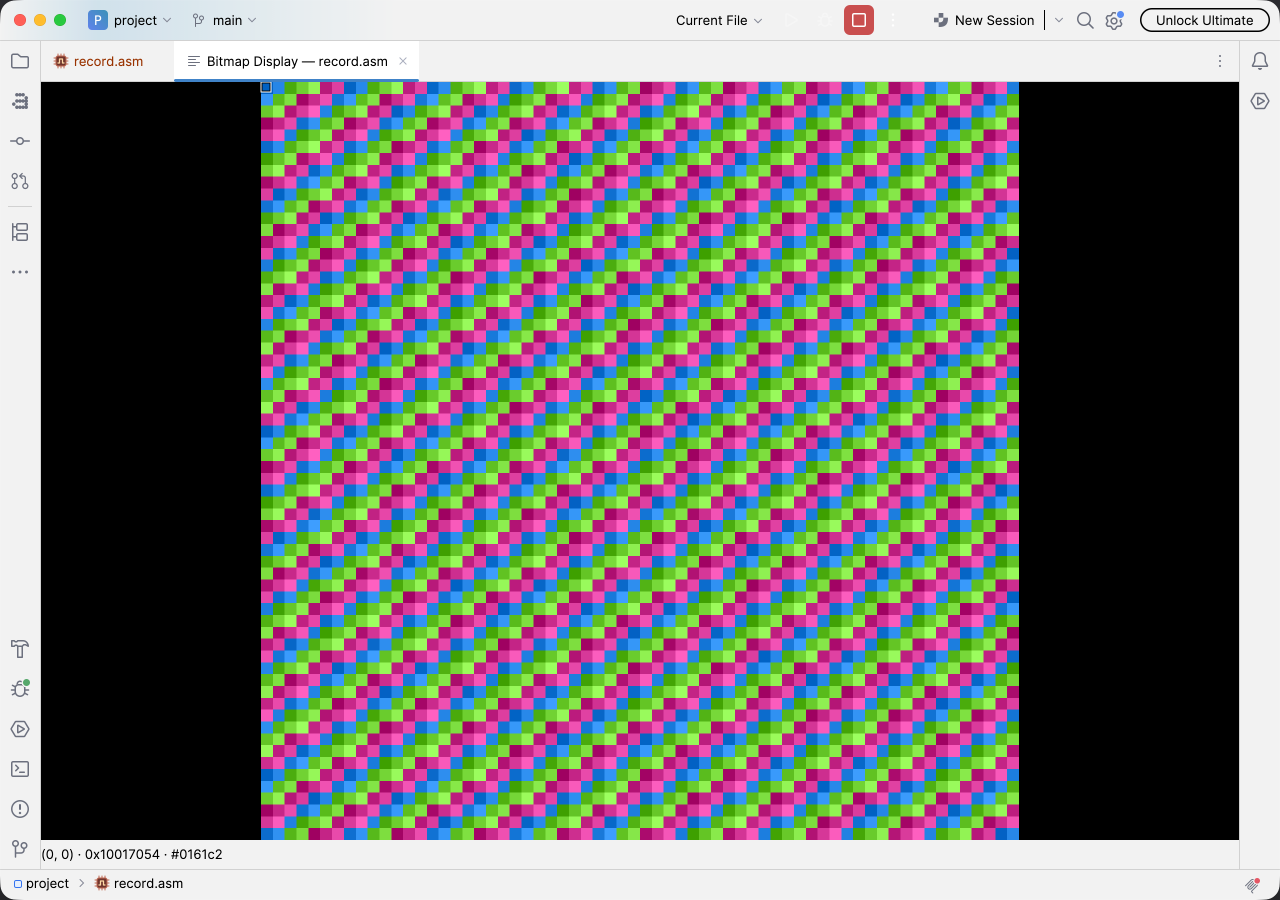
\includegraphics[width=0.47\linewidth,artifact,trim={\MARSrecordbitmapLeft{} \MARSrecordbitmapBottom{} \MARSrecordbitmapRight{} \MARSrecordbitmapTop{}},clip]{packages/034-lossless-video/captures/video-record-publication/bitmap.png}};
\begin{scope}[shift={(bitmap.south west)},x={($(bitmap.south east)-(bitmap.south west)$)},y={($(bitmap.north west)-(bitmap.south west)$)}]
\draw[black,line width=0.7pt] (0.007792208,0.007792208) rectangle (0.992207792,0.992207792);
\node[draw=black,fill=white,circle,inner sep=1.5pt,font=\footnotesize] at ($(0.007792208,0.992207792)+(-3mm,0)$) {2};
\end{scope}
\node[anchor=north west,inner sep=0,font=\small\bfseries] (context-title) at ([yshift=-3mm]bitmap.south west) {Retained and published context fields};
\node[anchor=north west,inner sep=0] (context) at ([yshift=-1mm]context-title.south west) {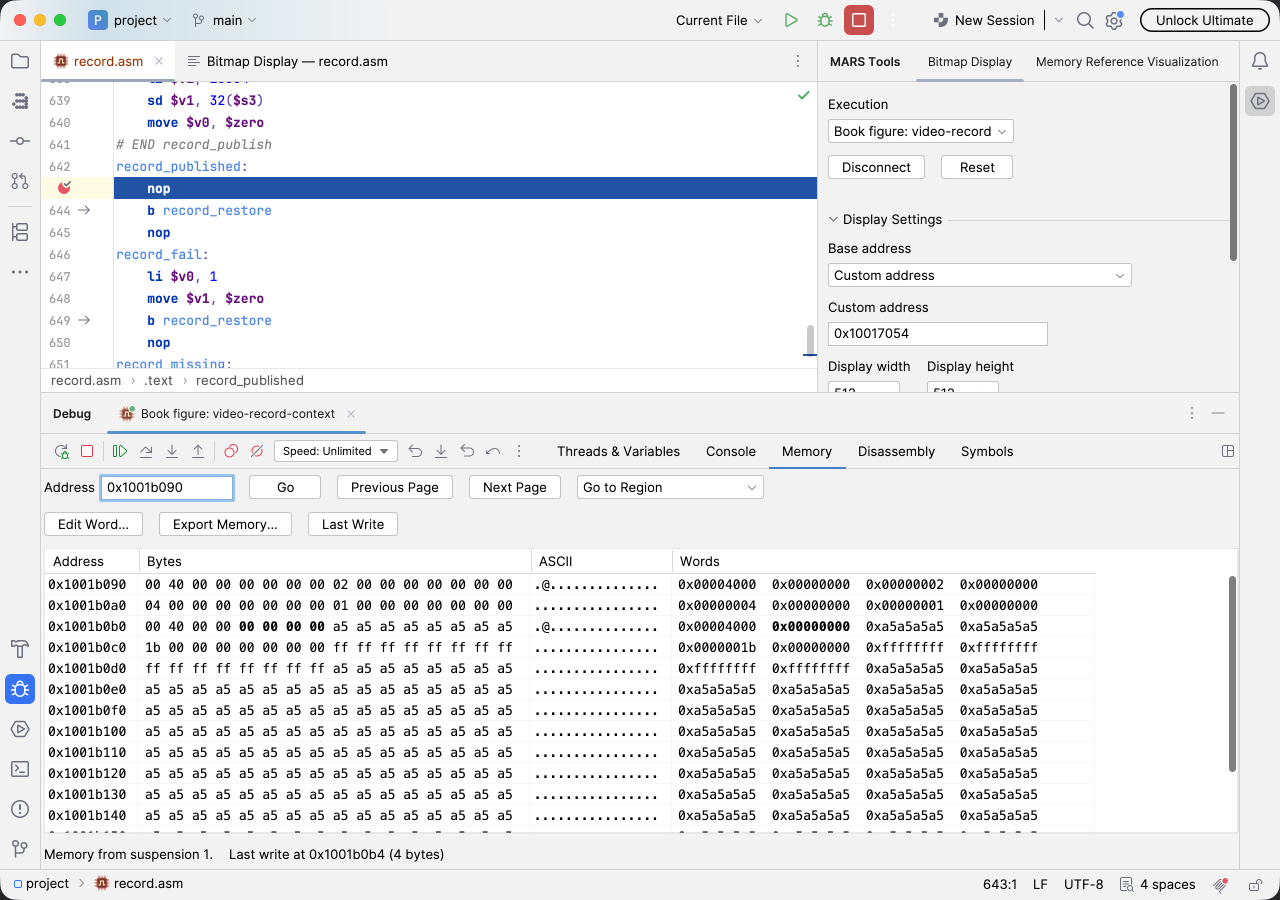
\includegraphics[width=0.74\linewidth,artifact,trim={\MARSrecordcontextLeft{} \MARSrecordcontextBottom{} \MARSrecordcontextRight{} \MARSrecordcontextTop{}},clip]{packages/034-lossless-video/captures/video-record-publication/context.png}};
\begin{scope}[shift={(context.south west)},x={($(context.south east)-(context.south west)$)},y={($(context.north west)-(context.south west)$)}]
\draw[black,line width=0.7pt] (0.013793103,0.043478261) rectangle (0.986206897,0.956521739);
\node[draw=black,fill=white,circle,inner sep=1.5pt,font=\footnotesize] at ($(0.013793103,0.956521739)+(-3mm,0)$) {3};
\end{scope}
\node[anchor=north west,inner sep=0,font=\small\bfseries] (returns-title) at ([yshift=-3mm]context.south west) {Success and active image size};
\node[anchor=north west,inner sep=0] (returns) at ([yshift=-1mm]returns-title.south west) {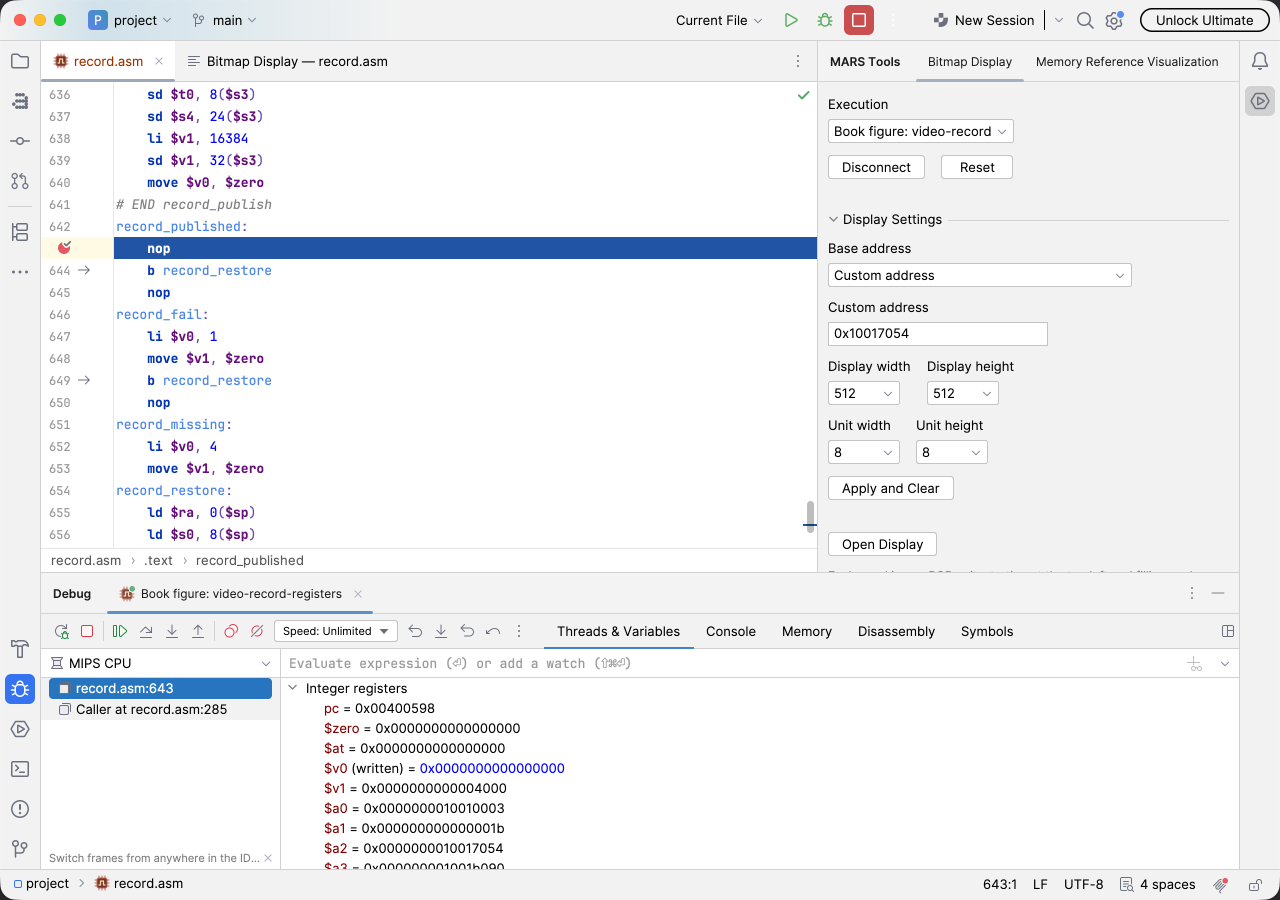
\includegraphics[width=0.5\linewidth,artifact,trim={\MARSrecordreturnsLeft{} \MARSrecordreturnsBottom{} \MARSrecordreturnsRight{} \MARSrecordreturnsTop{}},clip]{packages/034-lossless-video/captures/video-record-publication/registers.png}};
\begin{scope}[shift={(returns.south west)},x={($(returns.south east)-(returns.south west)$)},y={($(returns.north west)-(returns.south west)$)}]
\draw[black,line width=0.7pt] (0.023437500,0.045454545) rectangle (0.980468750,0.954545455);
\node[draw=black,fill=white,circle,inner sep=1.5pt,font=\footnotesize] at ($(0.023437500,0.954545455)+(-3mm,0)$) {4};
\end{scope}
\end{tikzpicture}
\par\smallskip
\begin{minipage}{\linewidth}
\small
\begin{enumerate}
\item The record has been accepted and its state published; the checkpoint \texttt{nop} has not executed.
\item The delta changes the initialized frame. Its first RGB word is now \texttt{0x000161c2}; the one-bit red change is too small to judge from the printed picture.
\item Read each 64-bit field as a low/high word pair in this little-endian run: capacity \texttt{0x4000}, next sequence two, period four, kind one, active bytes \texttt{0x4000}, and the retained \texttt{a5a5a5a5} suffix.
\item \texttt{\$v0} is zero; \texttt{\$v1} is \texttt{0x4000}, the 16\,384 bytes occupied by 4096 RGB words.
\end{enumerate}
\end{minipage}
\caption{A delta record accepted at the publication checkpoint. Three Debug launches show the same source, input and suspension point.}
\label{fig:video-record-publication}
\end{figure}
